\documentclass{sigchi}

% Use this command to override the default ACM copyright statement
% (e.g. for preprints).  Consult the conference website for the
% camera-ready copyright statement.


%% EXAMPLE BEGIN -- HOW TO OVERRIDE THE DEFAULT COPYRIGHT STRIP -- (July 22, 2013 - Paul Baumann)
% \toappear{Permission to make digital or hard copies of all or part of this work for personal or classroom use is      granted without fee provided that copies are not made or distributed for profit or commercial advantage and that copies bear this notice and the full citation on the first page. Copyrights for components of this work owned by others than ACM must be honored. Abstracting with credit is permitted. To copy otherwise, or republish, to post on servers or to redistribute to lists, requires prior specific permission and/or a fee. Request permissions from permissions@acm.org. \\
% {\emph{CHI'14}}, April 26--May 1, 2014, Toronto, Canada. \\
% Copyright \copyright~2014 ACM ISBN/14/04...\$15.00. \\
% DOI string from ACM form confirmation}
%% EXAMPLE END -- HOW TO OVERRIDE THE DEFAULT COPYRIGHT STRIP -- (July 22, 2013 - Paul Baumann)


% Arabic page numbers for submission.  Remove this line to eliminate
% page numbers for the camera ready copy

\pagenumbering{arabic}

% Load basic packages
\usepackage{balance}  % to better equalize the last page
\usepackage{graphics} % for EPS, load graphicx instead
%\usepackage[T1]{fontenc}
\usepackage{txfonts}
\usepackage{times}    % comment if you want LaTeX's default font
\usepackage[pdftex]{hyperref}
% \usepackage{url}      % llt: nicely formatted URLs
\usepackage{color}
\usepackage{textcomp}
\usepackage{booktabs}
\usepackage{ccicons}
\usepackage{todonotes}

% llt: Define a global style for URLs, rather that the default one
\makeatletter
\def\url@leostyle{%
  \@ifundefined{selectfont}{\def\UrlFont{\sf}}{\def\UrlFont{\small\bf\ttfamily}}}
\makeatother
\urlstyle{leo}

% To make various LaTeX processors do the right thing with page size.
\def\pprw{8.5in}
\def\pprh{11in}
\special{papersize=\pprw,\pprh}
\setlength{\paperwidth}{\pprw}
\setlength{\paperheight}{\pprh}
\setlength{\pdfpagewidth}{\pprw}
\setlength{\pdfpageheight}{\pprh}

% Make sure hyperref comes last of your loaded packages, to give it a
% fighting chance of not being over-written, since its job is to
% redefine many LaTeX commands.
\definecolor{linkColor}{RGB}{6,125,233}
\hypersetup{%
  pdftitle={HCI Final Paper},
  pdfauthor={Kyra Assaad, Zach Munro-Cape, Ajit Pawar, Ishan Thukral, \& Colin White},
  pdfkeywords={HCI, multitasking, application switching},
  bookmarksnumbered,
  pdfstartview={FitH},
  colorlinks,
  citecolor=black,
  filecolor=black,
  linkcolor=black,
  urlcolor=linkColor,
  breaklinks=true,
}

% create a shortcut to typeset table headings
% \newcommand\tabhead[1]{\small\textbf{#1}}

% For shared affiliation
\def\sharedaffiliation{%
\end{tabular}
\begin{tabular}{c}}
%

% End of preamble. Here it comes the document.
\begin{document}

\title{Multitasking Interfaces on Touchscreen Mobile Devices}

\numberofauthors{5}

%\author{
%    Kyra Assaad, Zach Munro-Cape, Ajit Pawar, Ishan Thukral, \& Colin White\\
%  \sharedaffiliation
%      \affaddr{Department Computer Science }  \\
%      \affaddr{University of Toronto }   \\
%      \affaddr{Toronto, Ontario} \\
%      \email{\{kyra.assaad, zach.munro.cape, ajit.pawar, ishan.thukral, colin.white\}@mail.utoronto.ca }
%}

\author{%
  \alignauthor{Ajit Pawar*\\
    \affaddr{University of Toronto}\\
    \affaddr{Toronto, Ontario}\\
    \email{ajit.pawar@mail.utoronto.ca}}\\
 \alignauthor{Colin White\\
    \affaddr{University of Toronto}\\
    \affaddr{Toronto, Ontario}\\
    \email{colin.white@mail.utoronto.ca}}\\
  \alignauthor{Ishan Thukral\\
    \affaddr{University of Toronto}\\
    \affaddr{Toronto, Ontario}\\
    \email{ishan.thukral@mail.utoronto.ca}}\\
 \alignauthor{Kyra Assaad\\
    \affaddr{University of Toronto}\\
    \affaddr{Toronto, Canada}\\
    \email{kyra.assaad@mail.utoronto.ca}}\\
  \alignauthor{Zach Munro-Cape\\
    \affaddr{University of Toronto}\\
    \affaddr{Toronto, Ontario}\\
    \email{zach.munro.cape@mail.utoronto.ca}}\\
}

\maketitle

*Authors arranged alphabetically by first name.

\section{Abstract}
Mobile smartphones are becoming more powerful, and multitasking on these devices is becoming more common. Being able to switch between applications quickly and accurately is essential to efficient performance on these devices. This study examines how different multitasking interfaces on a touchscreen mobile device (LG Nexus 5) affect performance time and accuracy when switching between open applications. Sixteen participants performed sets of tasks that involved varying levels of complexity when switching between applications on two different multitasking interfaces (stacked and non-stacked). They were monitored for speed and error rates. Results show that a stacked multitasking interface allows for slightly faster application switching as well as fewer errors when switching than with a non-stacked multitasking interface. This paper concludes with a discussion of our results, limitations to the study, and ideas for future research.

\section{keywords}
Multitasking; Task switching interfaces; Touchscreen; Mobile

\section{Introduction}

As smartphone technology has evolved, multitasking is now supported on many mobile devices. This allows users to have many applications (apps) running at once, and to switch between them to save startup time and state in a given app. Unlike PCs, screen real estate is much smaller on smartphones, meaning, for most devices, only one app can be in the foreground at a time. The ability to have one app open while launching another app is increasingly important for users to use their devices effectively. Leiva et al. estimate that app switching events are around 10\% of daily application usage [3]. Having multiple apps open at once is now commonplace and encouraged by device manufacturers and app developers. For example, you may draft an email, then switch to a photo editor, and then switch back to email to insert the edited photo into the draft.

The mechanism by which users switch active apps varies between devices. Lists of applications, search methods, or gestures are just some of the interactions to switch apps on smartphones. The most common way to switch apps is to open the application switching interface, or rather, the multitasking interface which varies by device. In the two major operating systems for smartphones, Android and iOS, each application is displayed in a list where the user can scroll through to select the desired application.

In this study, we aim to measure the app switching speed, accuracy, and perceived success of multiple methods for a user to switch to an already open app, perform a task, and then switch to another app in the Android operating system.

\section{Related Works}
The research on multitasking interfaces in smartphones is quite sparse. However, research has been conducted on the costs of interruption to a user's workflow when application switching, as well as designing more efficient multitasking interfaces for web and desktops.

Switching between apps incurs a cost in terms of task completion time. Nagata [5] examined the impact of digital interruptions on task performance on mobile and desktop devices, and Leiva et al. [3] studied the cognitive costs associated with switching apps. An interruption, say in the form of an app notification, can cause a user to multitask or switch apps by shifting attention from the task to the interruption [5]. Both studies found that task completion time increased when users switched between apps; in Leiva et al.'s study, that completion time was increased by a factor of four [3]. It was found that mobile web tasks with interruptions take longer to complete than on desktop, but when the interruption is expected, performance time decreased on a mobile device [5]. As a result, if a user is expecting to switch apps, they can complete tasks between apps more efficiently.

Given the cost to task completion time from switching apps, there have been many studies done on how to increase task resumption and completion time when multitasking. Leiva [2] explored different techniques to improve task resumption time in a multi-tab browser environment, and Lottridge et al. [4] investigated how the design of applications encourages or discourages multitasking behavior in general. Leiva investigated the effects of a tool designed to remind users of their position on the screen prior to app switching as well as the last interacted element and cursor position, while Lottridge et al. looked at making users more aware of the time spent in "work" versus "non-work" categories of websites. Lottridge et al. found that by making users more aware of the passage of time, users had fewer webpage tabs open, fewer tab switches and shorter sessions within webpages [4], indicating that users were more efficient with their time spent on the web. Leiva found that the use of his tool improved task resumption time and task completion time.

Card and Henderson [1] observed that users interacting with an interface often organize tasks along a number of different dimensions, the most important of them being "locality" of tasks. The study found that users often form clusters of windows corresponding to a specific task. This insight led to development of interfaces that produce "virtual views" that allow users to focus their interactions within semantically meaningful clusters of windows. Modern smartphone multitasking interfaces sort opened apps in chronological order, but if a user is switching between two or three apps a time to perform a task, those apps in smartphone multitasking interfaces will be sorted together at the front of the list. If the apps are "clustered" to match with the user's mental model, this could result in faster and less error-prone application switching. In fact, Oliver et al. investigated a tool that indicated which windows in a multitasking interface were semantically related [6]. The use of this tool resulted in significantly more efficient task completion time, but it was noted that there was a negative effect when windows in the multitasking interface were reordered if the user interrupted the main task to switch to a different task [6]. This is what currently occurs in smartphone multitasking interfaces, which is why we intend to investigate the speed and accuracy of modern smartphone multitasking interfaces.

In the study that is most closely related to this experiment, Warr and Chi [7] explored whether a "cards"-based mobile webpage switcher, which stacks open webpages like cards in the display, would result in faster webpage switching and less errors than a "pages"-based switcher, where the webpages are displayed as pages laid out next to each other. The research revealed that it is faster to switch webpages in the cards-based interface compared to the pages-based interface, but that there was no significant difference in error rates between the two interfaces [7]. These authors were specifically investigating a web browser switching interface and that was across two different operating systems. Our experiment is on one operating system, and focuses on speed and error rate difference between two common multitasking interfaces.

\section{Research Question and Hypotheses}
The purpose of this experiment is to determine how, if at all, different mobile multitasking interfaces affect accuracy in switching between applications as well as the time that it takes to switch applications. We will be investigating two different interfaces: a stacked interface where the pages that represent different opened apps overlap with each other, and a non-stacked interface where the pages are separated. \\

H1: Users will be faster at switching between applications in the stacked interface.\\
H2: Users will have greater accuracy when switching between applications in the non-stacked interface. \\

The reasoning behind this is that while there can be more applications visible at any given time in a stacked layout, each application has a smaller target area to select, which translates into less accuracy.

\section{Methodology}
\subsection{Apparatus}
Two LG Nexus 5 phones were used as the apparatus for the experiment, one loaded with the stacked multitasking interface and the other with the non stacked interface. The stacked interface uses Android OS version 5.1 (Lollipop) while the non-stacked uses Android OS 4.4.4 (KitKat). Both Android OS versions used were official Google releases and did not include any carrier or manufacturer modifications.

The Nexus 5 was released two years ago and has a 4.95 inch screen with a Snapdragon 800 Quad-Core processing chip. These specifications put it in the mid-range of current Android phones. We felt that using the Nexus 5 gives us a more accurate representation of what an average Android user would be using in the real world. This will reduce the bias of unfamiliarity and novelty when testing.

\begin{figure}
 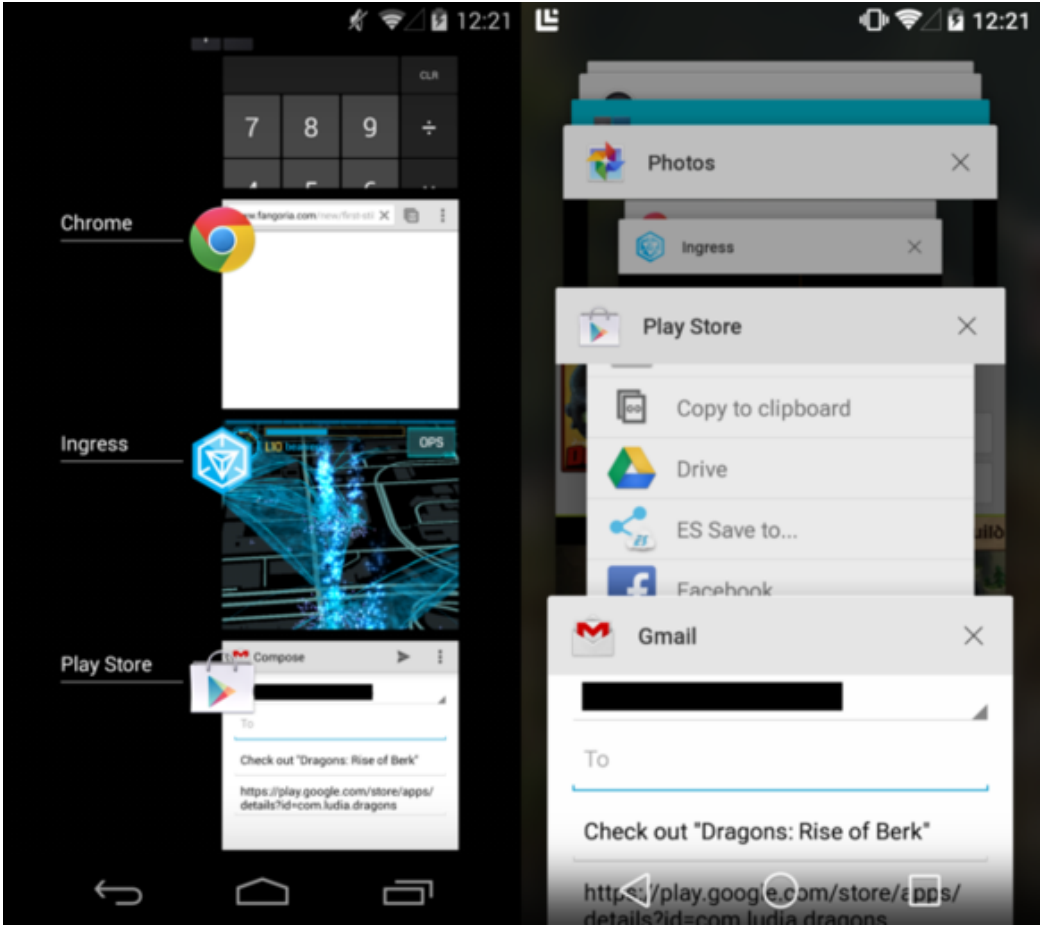
\includegraphics[width=\linewidth]{img/layout_no_cap.png}
 \caption{Left: The non-stacked multitasking interface of Android 4.4 KitKat. Right: The stacked interface of Android 5.0 Lollipop.}
\end{figure}

\subsection{Participants}
Sixteen participants (ages 19-26) were recruited and did not receive monetary compensation for their participation. They all were currently pursuing an undergraduate degree at the University of Toronto. All participants met the criteria of previous experience with the Android operating system and no visual or hand dexterity disabilities. Participants were randomly assigned to begin with the stacked interface (n=8) or non-stacked interface (n=8). The study was carried out in a meeting room at the Mobile Application Development Lab (MADLab) which is located at the University of Toronto.

\subsection{Experimental Design}
The experiment had a one-way within-subject design with the multitasking interface (stacked and non-stacked) acting as a two-level independent variable. Order effects were counterbalanced by switching the order of testing with two groups of participants. The first group tested the stacked interface first on the Lollipop phone, while the second group tested the non-stacked interface first on the KitKat phone. Time to completion and accuracy served as the dependent variables. Participants performed the set of tasks twice for each stacked and non-stacked multitasking interfaces with two different experimenters.

Randomizing participants into groups allowed us to minimize the variance any participants may have had in terms of greater experience or comfort with one interface over the other. Since the experimental tasks are repetitive, the participants were susceptible to the learning-effect. However, counterbalancing based on the two levels of the independent variable allowed us to account for it.

\subsection{Tasks and Procedures}
The experimenter explained the purpose of the experiment to the participant and answered any general questions about the experiment. Each participant completed the entry survey and signed the consent form. The participants were free to withdraw at any point during the experiment. The experimenter showed the participant the experimental setup and described the tasks. For the setup, the experimenter confirmed that the phone was set up for each task, and that both phones were plugged into a computer and were being monitored. The experimenter confirmed that the participant knew how to open the multitasking interface and use the copy and paste function on the phone.

Each task was designed to cover one of three common interactions. First was a minimal interaction, where the application switches was limited to one or two switches between three open applications. Second was a longer task where the participant switched between three or more applications. In this task, participants had to scroll through the multitasking interface, which presented a non-ordered list of apps to find the app they were to switch to. Last was a repetitive switching task, a common scenario where the participant repeatedly switched between two apps to achieve a specified goal. Combined with a within-subject design where the participant performs these tasks multiple times on each level gave us a comprehensive set of data points to test the hypotheses. 

Each participant executed each block twice, once on each multi-tasking interface (stacked and non-stacked). There were six trials in total per participant. Each participant was handed a sheet outlining all the tasks for each block. Each block of tasks was preceded by a short break for the experimenter to setup the device and demonstrate the tasks, if requested by the participant. Participants were instructed to begin tasks and were observed for any errors. Errors were recorded as a total per task block. Tasks were completed at the participant's? own pace and errors (if any) were corrected at their discretion. Experimenter logged the data for each block of tasks on each interface. At the commencement of the experiment, the participant completed an exit survey. The whole experiment took about 20 minutes to complete per participant.

\subsection{Measures}
The dependent variables in this study were time spent in the multitasking interface, which corresponds to time taken to switch between apps, and the  accuracy when switching apps. Time to completion is measured as when the participant opens the multitasking interface to when the participant opens the target app. Accuracy is defined as when a participant does not open the target app in the task and instead either opens a different app or goes to the home screen. Measuring time to completion and accuracy will show which interface allows for fastest and least error-prone application switching.

\subsection{Data Collection}
Each participant completed a short questionnaire before the experiment to determine age, gender, handedness, prior experience with Android, whether they owned an Android phone, and which OS version they were most comfortable with. Another questionnaire was completed after the experiment to determine perceived speed and accuracy with the two multitasking interfaces, as well as general preference for one interface over another. During the experiment, the Android phones were connected to a MacBook Pro via micro-USB cable. Task completion time was logged using the Android Debug Bridge logging system. Errors were monitored by the experimenter and made note of. The task logs were parsed using a Python script, and the data was outputted in ANOVA readable format.

\section{Results}
The mean task completion time for each participant on each interface is outlined in the following table.

%\begin{center}
% \begin{tabular}{|c c c|}
% \hline
% Participant Number & Kitkat Speed & Lollipop Speed \\ [0.5ex]
% \hline\hline
% 1 & 2.52 & 2.19\\
% \hline
% 2 & 2.46 & 2.59 \\
% \hline
% 4 & 2.28 & 2.14 \\
% \hline
% 5 & 2.80 & 3.27 \\
% \hline
% 6 & 2.76 & 2.17 \\
% \hline
% 7 & 1.96 & 1.89 \\
% \hline
% 8 & 2.02 & 1.79 \\
% \hline
% 9 & 2.60 & 2.67 \\
% \hline
% 10 & 2.06 & 1.17 \\
% \hline
% 11 & 2.95 & 1.87 \\
% \hline
% 12 & 2.28 & 1.71 \\
% \hline
% 13 & 2.88 & 1.85 \\
% \hline
% 14 & 1.92 & 2.72 \\
% \hline
% 15 & 2.05 & 2.46  \\
% \hline
% 16 & 2.69 & 3.03 \\
% \hline
%  17 & 1.73 & 2.00 \\
% \hline \hline
% Avg & 2.37 & 2.22 \\
%
% \hline
%\end{tabular}
%\end{center}

Given that this was a within-subjects test with one independent variable, a one-way with one within-subjects factor ANOVA test was carried out.
The mean task completion times was 2.37 seconds for the non-stacked interface (KitKat). This was 6.7\% slower than the mean of stacked interface (Lollipop) which was 2.22 seconds. The difference was not statistically significant.

\begin{center}
$(F_{1, 15} = 1.19, ns )$
\end{center}

The number of errors per device over the testing period is presented below.

%\begin{center}
% \begin{tabular}{|c c c|}
% \hline
% Participant Number & Kitkat Errors & Lollipop Errors \\ [0.5ex]
% \hline\hline
% 1 & 1 & 1\\
% \hline
% 2 & 10 & 5\\
% \hline
% 4 & 0 & 0 \\
% \hline
% 5 & 1 & 3 \\
% \hline
% 6 & 4 & 1 \\
% \hline
% 7 & 0 & 2 \\
% \hline
% 8 & 0 & 1 \\
% \hline
% 9 & 10 & 4 \\
% \hline
% 10 & 1 & 0 \\
% \hline
% 11 & 2 & 2 \\
% \hline
% 12 & 3 & 3 \\
% \hline
% 13 & 1 & 1 \\
% \hline
% 14 & 0 & 0 \\
% \hline
% 15 & 1 & 0  \\
% \hline
% 16 & 2 & 1 \\
% \hline
%  17 & 2 & 1 \\
% \hline \hline
% Avg & 2.37 & 1.56 \\
%
% \hline
%\end{tabular}
%\end{center}

The mean error rate for was 2.37 errors for the non-stacked interface and 1.56 errors for the stacked interface. However, as there was substantial variation in the errors across participants, the difference was not statistically significant as revealed by the analysis of variance. Once again, a one-way with one within-subjects factor ANOVA test was carried out.
\begin{center}
$(F_{1, 15} = 2.19, ns )$
\end{center}

The exit survey questions relating to the participant�s perceived accuracy and speed were converted to an ordinal scale between 1 and 5. Participants believed they were slightly faster on the stacked interface (3.92 average response versus 3.76). Participants perceived they were more accurate on the non-stacked interface (4.38 average response versus 4.07).

\section{Discussion}
While the trends in the speed and accuracy measurements of our participants was statistically insignificant between the two interfaces, a discussion can still take place. The stacked interface was perceived by the participants to be faster, which held when examining the data. This is inline with previous research, such as the work of Warr and Chi [7]. However, a follow-up question is presented: why is stacked interface perceived as quicker? It?s possible this is due to the fact that the motion of the cards is toward the user rather than down. In addition, with the stacked interface the user can control the sensitivity of the scroll by scrolling from higher up on the screen. This allows users to more quickly traverse a long list of apps at the cost of some granularity of motion.

\section{Conclusion}
Overall, the experiment showed that the differences between the two interfaces are statistically insignificant for accuracy and speed. The stacked  interface was rated as generally more pleasant and quicker, which could be a reason Google updated Android?s default multitasking interface.

One limitation of our participant group was their familiarity with the two operating systems. From the starting survey 9 participants were mostly familiar with Lollipop whereas only 3 were mostly familiar with KitKat. Another limitation is that the study only tested one model of phone with stock Android. The real consumer landscape for Android contains many different sized phones running various modified versions of Android.

A stacked interface may only provide nominal speed and accuracy increases when compared to a non-stacked interface. As a result, future research should focus on alternate means to facilitate app switching as opposed to the conventional chronological list of applications. Throughout all mobile multitasking interfaces, almost exclusively, the "most recently used" rule is used to display applications in the list. Future research could look into using different sorting schemes to predict which application a user will need next. Perhaps machine learning could be applied to predict what application may be used next as is being tested in Apple?s new recents menu.

\section{References}
1. Card, S. and Henderson Jr., A. A multiple, virtual-workspace interface to support user task switching.  \textit{Proceedings of the SIGCHI/GI Conference on Human Factors in Computing Systems and Graphics Interface}, CHI '87 (1986), 53-59.

2. Leiva, L. MouseHints: easing task switching in parallel browsing.  \textit{CHI '11 Extended Abstracts on Human Factors in Computing Systems}, CHI EA '11 (2011), 1957-1962.

3. Leiva, L., B�hmer, M., Gehring, S. and Kr�ger, A. Back to the app.  \textit{Proceedings of the 14th international conference on Human-computer interaction with mobile devices and services}, MobileHCI '12 (2012), 291-294.

4. Lottridge, D., Marschner, E., Wang, E., Romanovsky, M. and Nass, C. Browser Design Impacts Multitasking.  \textit{Proceedings of the Human Factors and Ergonomics Society Annual Meeting 56}, 1 (2012), 1957-1961.

5. Nagata, S. Multitasking and Interruptions during Mobile Web Tasks.  \textit{Proceedings of the Human Factors and Ergonomics Society Annual Meeting 47}, 11 (2003), 1341-1345.

6. Oliver, N., Czerwinski, M., Smith, G. and Roomp, K. RelAltTab.  \textit{Proceedings of the 13th international conference on Intelligent user interfaces}, IUI '08 (2008), 385-388.

7. Warr, A. and Chi, E. Swipe vs. scroll.  \textit{Proceedings of the SIGCHI Conference on Human Factors in Computing Systems}, CHI '13 (2013).

\end{document}

%%% Local Variables:
%%% mode: latex
%%% TeX-master: t
%%% End:
